\documentclass[a4paper]{article}
\usepackage{INTERSPEECH2015,amssymb,amsmath,epsfig, epstopdf}
%\usepackage[named]{algo}
%\usepackage[numbered]{algo}
\setcounter{page}{1}
\sloppy     % better line breaks
\ninept 
%SM below a registered trademark definition
\def\reg{{\rm\ooalign{\hfil
     \raise.07ex\hbox{\scriptsize R}\hfil\crcr\mathhexbox20D}}}

%% \newcommand{\reg}{\textsuperscript{\textcircled{\textsc r}}}
\title{Confidence-Features and Confidence-Scores for ASR applications in Arbitration and DNN Speaker Adaptation}

%%%%%%%%%%%%%%%%%%%%%%%%%%%%%%%%%%%%%%%%%%%%%%%%%%%%%%%%%%%%%%%%%%%%%%%%%%
%% If multiple authors, uncomment and edit the lines shown below.       %%
%% Note that each line must be emphasized {\em } by itself.             %%
%% (by Stephen Martucci, author of spconf.sty).                         %%
%%%%%%%%%%%%%%%%%%%%%%%%%%%%%%%%%%%%%%%%%%%%%%%%%%%%%%%%%%%%%%%%%%%%%%%%%%
%\makeatletter
%\def\name#1{\gdef\@name{#1\\}}
%\makeatother
%\name{{\em Firstname1 Lastname1, Firstname2 Lastname2, Firstname3 Lastname3,}\\
%      {\em Firstname4 Lastname4, Firstname5 Lastname5, Firstname6 Lastname6,
%      Firstname7 Lastname7}}
%%%%%%%%%%%%%%% End of required multiple authors changes %%%%%%%%%%%%%%%%%

\makeatletter
\def\name#1{\gdef\@name{#1\\}}
\makeatother \name{{\em Kshitiz Kumar, Ziad Al Bawab, Yong Zhao, Chaojun Liu, Benoit Dumoulin, Yifan Gong}}

\address{Microsoft Corporation, Redmond, WA \\
{\small \tt \{Kshitiz.Kumar, Ziadal, Yonzhao, Chaojunl, Bedumoul, Yifan.Gong\}@microsoft.com}}

%
\begin{document}
\maketitle

\begin{abstract}
Speech recognition confidence-scores quantitatively represent the correctness of
decoded utterances in a [0,1] range. Confidences have primarily been used to filter out recognitions with scores below a threshold. They have also been used in other speech applications in \emph{e.g.} Arbitration, ROVER and high-quality data selection for model training etc. Confidence-scores are computed from a rich set of confidence-features in the speech recognition engine. While many speech applications consume confidence scores, we haven't seen adequate focus on directly consuming confidence-features in applications. In this work we build a thesis that additionally consuming confidence-features can provide big gains across confidence-related tasks. We demonstrate this for Arbitration application, where we obtain 31\% relative reduction in arbitration metric. We additionally demonstrate a novel application of confidence-scores in deep-neural-network (DNN) adaptation, where we can nearly double the relative reduction in word-error-rate (WER) for speaker adaptation on limited data.
\end{abstract}
\noindent{\bf Index Terms}: Speech recognition, Confidence scores, Confidence predictors, Classifier, MLP

%
\section{Introduction}\label{Sec:Intro}
Automatic speech recognition (ASR) has seen a huge wave of deployment and usage across devices and services in recent years.
Confidence-scores are integral component of ASR, these scores quantify the correctness of recognition results. Historically confidences were used for ASR-enabled devices that are always in an active (continuously) listening mode in an application-constrained grammar. There potential recognitions from side-speech, background noise etc. can trigger unexpected system response. Therefore, it's critical to prevent out-of-grammar (OOG) utterances from being recognized as in-grammar (IG) utterances.
Confidence-scores are typically evaluated for a word as well as for an utterance.

Recently confidence-scores have also been used in other ASR applications in (a) system combination using ROVER, (b) selecting one of client or service recognition in Arbitration, (c) selecting high-quality data for unsupervised model training, (d) Key-word spotting, (e) confidence-normalization etc. While many of the downstream speech applications consume confidence-scores we have seen limited attempts on additionally consuming confidence-features. In this work we present our individual confidence-features, and, discuss the diverse information that they capture. We specifically demonstrate the richness of these features for Arbitration application where we present significant gains in arbitration metric. We also present a DNN speaker adaptation application where we include confidence-scores in adaptation framework.


The confidence classifier is trained to maximally discriminate between correct and incorrect
recognitions. Confidence scores lie in a [0,1] range, we desire higher scores for correct recognitions, and lower for,
(a) incorrect recognitions from in-grammar and, (b) any recognition from out-of-grammar utterances.
The classifiers are trained from a specified set of acoustic model (AM), grammar and speech data, this establishes classifier
profile in terms of CA and FA at different thresholds. We associate an operating threshold with
the classifier and accept recognitions with scores greater than the threshold, upon which we evaluate correct-accept (CA) and false-accept (FA) measures.

We refer \cite{Posen1} for an introduction to our confidence classifier framework. There we
also discussed our predictors confidence classifier approaches.
We refer \cite{CMsurvey_Jiang_SpeechCommunication06, NBest_Wessel_Eurospeech99, MaximumEntropyConfidence_White_ICASSP07,Blatz04confidenceestimation,Rose_UV_1995,Mathan_Rejection_1991,Sukkar_UV_1996}
for a survey of other confidence techniques and specifically \cite{WordLattice_Kemp_Eurospeech97, MaximumEntropyConfidence_White_ICASSP07, Wessel01ney,Chase_wordand,Weintraub97}
for predictors and the classifiers used.

Rest of this work is organized in the following. We explicitly discuss the relevance of 
confidence normalization in Sec.~\ref{sec:ConfNorm}. We present confidence normalization techniques in Secs.~\ref{sec:hist-map}, ~\ref{sec:poly-map},~and \ref{sec:tanh-map} and present 
related experiments and results in Sec.~\ref{sec:results}. Sec.~\ref{sec:conclusion} concludes this study.


\section{Background on Confidence-Features and Confidence-Scores}\label{Sec:CC-Background}
We discussed the significance of confidence-score in Section~\ref{Sec:Intro} where we mentioned the job of the 
confidence-classifier is to make an inference on the correctness of recognition events. This is thus a binary
classification problem \cite{Bishop} with the 2-classes in (1) correct recognitions, (2) all incorrect
recognitions that includes misrecognitions over IG utterances as well any recognition
from OOG utterances. The classifier is trained from a rich set of confidence-features that we obtain from speech decoding.
Some of the prominent features are:
\begin{enumerate}
  \item acoustic-model features - we aggregate per-frame acoustic score over a word or an utterance. We also compute scores from acoustic arc transitions. These scores are typically normalized with respect to duration and 
  \item language-model features - we compute language fanout, perplexity
  \item noise and silence-model features - we compute features from noise and silence models
  \item 2nd order features - we can compute weighted average of above features with respect to words in a phrase
  \item duration features - we can compute number of words in a phrase, word-duration etc.
\end{enumerate}
Some other features may include count of senones from decoding. Above features are appropriately normalized to be robust to speech with different duration and intensity. Though confidence-scores have been used in a number of speech applications, we have seen limited focus on directly consuming confidence-features in the applications. The count of these features is typically 15-20 for a word or for an utterance, so additional memory required to store these features is minimal. Most of the current ASR engine just output recognition text along with confidence. These confidence-features are already computed for the purpose of confidence-score so there is almost no additional work required for extracting confidence-features. Furthermore, these confidence-features also need to be transferred alongwith ASR result to the consumer to these features. Considering a typical speech segment of 4 seconds encoded at 8 kB/second for a total of 32kb, confidence-features just add 60 Bytes to the footprint, thus less than 0.2\% to overall footprint.

We set up a large pool of training data, grammar, and obtain positive tokens from successfully recognized utterances and negatives from wrong recognitions. Based on above set of positive and negative features, we build a multi-layer perceptron based classifier (MLP) \cite{Mathan91, Bishop}. This uses a single hidden layer with specified set of nodes and is trained with mean-squared error (MSE) criterion. We can build a classifier for either word or sentence. For word classifier, predictors are aggregated and averaged across a word boundary, similarly predictors are aggregated over a sentence for corresponding classifier.
Our confidence-features consist of 16 individual features. We refer to \cite{Posen1} for additional details on our confidence classifier architecture.


\section{Rich Confidence-Features for Arbitration}\label{Sec:Arbitration}
Arbitration is an application where we expect to select the best among one of the multiple simultaneous ASR results.
We explain our arbitration framework for Microsoft Cortana experience on smart devices in Fig.~\ref{Fig:Arbitration}, where we simultaneously decode an utterance against both client and service engines, and select the best result. Client engine is designed to work with traditional client scenarios like \emph{call, digit dialing, text, open applications etc.}, service engine works for rest of the speech scenarios including \emph{voice-search, weather etc.}. By design the client and service cater to distinct speech scenarios and contain language-model and acoustic-model optimized for those tasks. Though we have distinct engines for client and service speech scenarios, they work together in a unified way that is indistinct for the user as we obviously don't expect user to provide us inputs on his scenario being one of client or service. Arbitration is the key speech application that provides a unified experience by selecting the best among the client and service results.  Both client and service listen to speech from potentially all scenarios and produce respective recognition results under the constraint of their respective engine, AM and LM. These results are communicated to arbitration where it selects the best between the 2 results. Arbitration then sends the results back to client where a decision unit at client will typically provide the arbitrated result to the user on their smart devices.

There can be a few scenarios where the decision unit can simply choose the client recognition \emph{e.g.}, (a) if the client confidence-scores are higher than a present threshold - typically the process of getting the arbitrated ASR result back from service may incur some latency so client can simply choose client ASR result if it's very confidence about it, (b) absence of connection to service - in these cases user can still make use of client side speech applications from Microsoft or other $3^{rd}$-party applications. 

% This framework also allows us to cater to scenarios where a user says: ``text Alex, I will be late". There client engine has access to contacts and can recognize the person name ``Alex" and produce a result like ``text Alex ...", then ``..." will be filled in by recognition from service. Client AM contains garbage paths that greatly help absorb utterances are intended for service only and thus are out-of-grammar (OOG) for client.

\subsection{Arbitration Classifier and Baseline Features}\label{Sec:ArbitrationCC}
Brief description of current arbitration framework, and current useful features

\begin{figure}[h]
\centering
{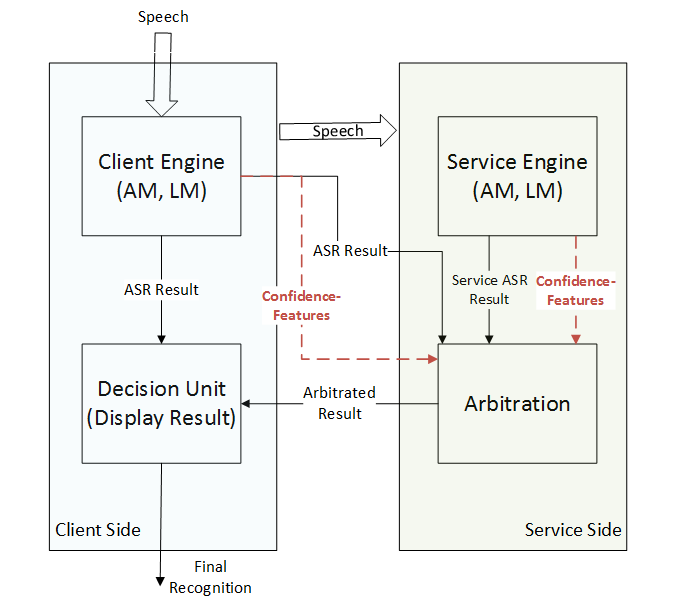
\includegraphics[width=0.47\textwidth]{Arbitration}}
\caption{\it Arbitration for client and service ASR resuls.}
\label{Fig:Arbitration}
\end{figure}

\subsection{Incorporating Confidence-Features in Arbitration}
We described our arbitration framework and the baseline features in \ref{Sec:ArbitrationCC}, there we mentioned a number of features that we found very relevant for arbitration. In this section, we build a thesis on consuming the rich set of confidence-features in arbitration. We first note that although our arbitration baseline features provide very useful information, the confidence-features provide detailed information in noise, silence, acoustic and language-model scores, all this is expected to useful for arbitration. We also note that although confidence-scores from both client and service is used by arbitration that are expected to provide a good gist of confidence-features, we can still benefit a great deal with directly consuming confidence-features by, (a) using much more gradual information in terms of 15-20 confidence-features vs. a single confidence-score, (b) confidence-scores are designed to optimize the performance confidence-classifier which is clearly different from arbitration, so retraining with confidence-features can help, (c) arbitration and confidence-classifier may be trained over different datasets, so the information encapsulated by confidence-score may not generalize to dataset relevant for arbitration, (d) confidence-scores are language-specific as they may have been individually trained across a set of \emph{AM, LM, languages, dataset}, in contrast, we have noted that the various inherent normalizations in confidence-features make them robust across locals, so consuming confidence-features can allow us to build an arbitration classifier from one local that can provide good performance for other unseen locals, this can be specially useful when we may need to bootstrap arbitration from a local under limited data scenarios, (e) using confidence-score in arbitration creates a dependency for arbitration on confidences, any update to confidence-classifiers potentially requires retraining arbitration, we can alleviate this issue if we directly consume confidence-features while not using confidence-score in arbitration, this decouples arbitration and confidence-classifiers, letting us independently update confidence-classifier without impacting arbitration.

We demonstrate our approach that uses the rich confidence-features for arbitration in Fig.~\ref{Fig:Arbitration}. We build the infrastructure required to extract confidence-features from both client and service engine, and communicate them to arbitration, see Fig.~\ref{Fig:Arbitration}. As expected we require little additional additional work in communicating service confidence-features to arbitration. For client, we additionally send about 30 Bytes-per-second of data, this is less than 0.2\% relative increase to our payload from client to service. Depending on application and need, arbitration can be retrained and deployed with confidence-features from (a) just client, (b) just service, (c) both client and service. 

% 3 second, 20 float features = 20 * 4 = 80 bytes = 30bytes/sec
% speech data = 8000 bytes

\subsection{Arbitration Experiments and Results}\label{Sec:ArbitrationResults}
We present and analyze results from using confidence-features in arbitration as discussed in Sec.~\ref{Sec:Arbitration}.
Our arbitration was trained from over 35k speech utterances. Testing was done on over 25k utterances. 
We decoded these utterances against both client and service engines with their respective  AM and LM, and obtained corresponding recognition results. We had ground-truth transcriptions for these utterances and created their classification targets in terms of client or service based on WER criterion. We obtained the arbitration baseline-features that included confidence-score, and additionally obtained confidence-features from both client and service. Note that ideally clients will have distinct personalized grammars with their own contact names, application names etc. For our purposes we simulated client grammar with each over 250 names in contacts and used these grammars in decoding. We followed the existing framework for training arbitration classifier where we additionally included confidence-features.

Next, we demonstrate the value in client confidence-features in Fig.~\ref{Fig:PhrasePreds-Hist}, there we plot features distribution for a few features for arbitration task. There ``correct" refers to cases where client wins, and ``InCorrect" refers to service wins, ``Confidence-Score" indicates usual client confidence-score. We visually see that some of the features much better separate the 2 classes than confidence-score.

\begin{figure}[h]
\centering
{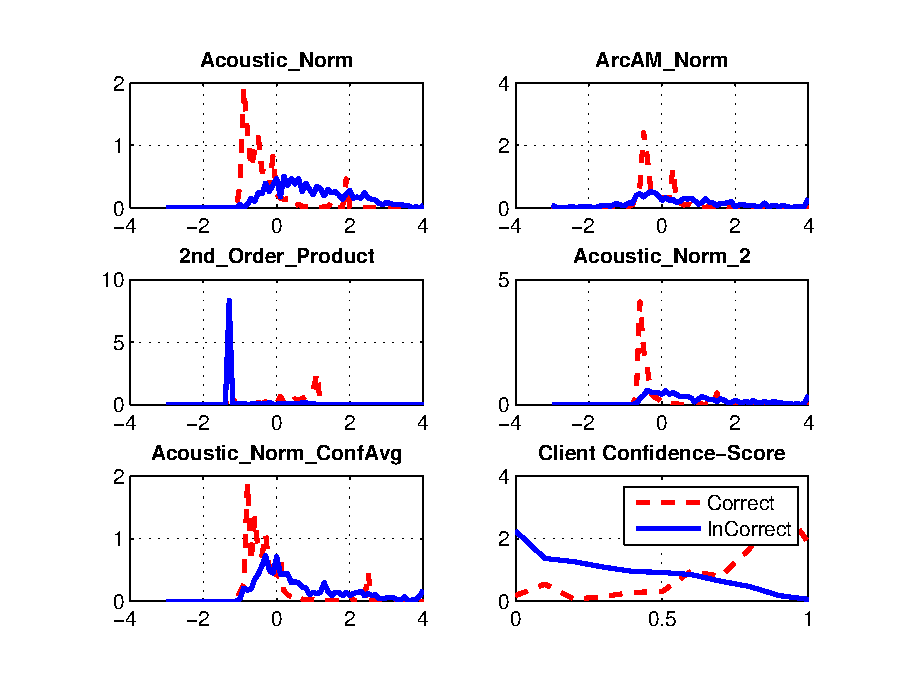
\includegraphics[width=0.5\textwidth]{PhrasePreds-Hist.eps}}
\caption{\it Mapping to normalize confidences.}
\label{Fig:PhrasePreds-Hist}
\end{figure}

Next we provide receiver-operating-curve (ROC) for baseline and with including client confidence-features in Fig.~\ref{Fig:Baseline-ClientPred-ROC}, where we note a strongly better ROC curve throughout the range of curve. In this arbitration task, ``False Positive" (FP) indicates incorrect wins from client and ``True Positive" (TP) indicates correct wins from service. Specifically at FP of 0.1, we can improve TP from 0.81 to 0.86, for a 26\% relative reduction in (1-TP). We note correct area-under-the-curve (AUC) metrics in Table~\ref{tab:AUC_ROC}, where including client confidence-features improved AUC from 0.927 for baseline to 0.946, additionally including server confidence-features improved AUC to 0.95 for a 31.5\% relative reduction in (1-AUC) metric.

\begin{figure}[h]
\centering
{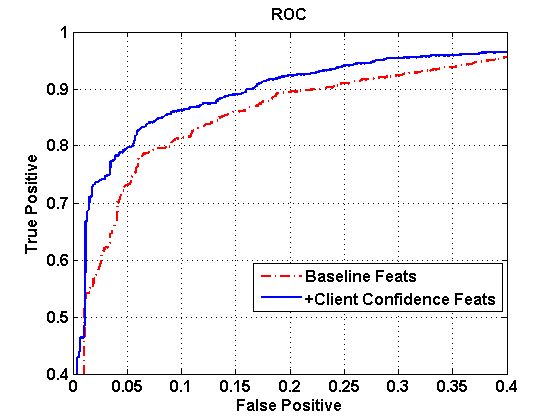
\includegraphics[width=0.47\textwidth]{Baseline-ClientPred-ROC}}
\caption{\it Mapping to normalize confidences.}
\label{Fig:Baseline-ClientPred-ROC}
\end{figure}

\begin{table}
\begin{center}
\begin{small}
\caption{Area-under-the-curve (AUC) for ROC chart} \label{tab:AUC_ROC}
\begin{tabular}{|l|c|c|}
\hline
Method & AUC & relative reduction in \\
& & (1-AUC) [\%]\\
\hline
Baseline Features & 0.927 & - \\
\hline
+ Client Confidence-Features & 0.946 & 26.0\\
\hline
+ Client and Service & &\\
~~Confidence-Features & 0.950 & 31.5\\
\hline
\end{tabular}
\end{small}
\end{center}
\end{table}

Our arbitration classifier ranks all of it's features in the order of importance. As expected confidence-features appear prominently among the top features, with 7 of the top-10 overall features being confidence-features. This further demonstrates that the proposed features outperform and add value to the baseline features.


\section{Confidence-Scores in DNN Speaker Adaptation Framework}\label{Sec:Adaptation}
In this sec. we present a new application of confidence-scores in the DNN adaptation framework. We have huge gains in WER across many scenarios with the deployment of DNNs but we have also established that speaker adaptation of DNN models provides a significant scope for further improvements. In this section, we present our baseline speaker adaptation approach and propose to additionally include confidence-scores in speaker adaptation with limited and large adaptation data scenarios. We have noted that confidence-scores imply the correctness of recognition results. In the context of speaker-adaptation confidence-scores also indicate a degree of match between the speaker-dependent data and speaker-independent model, thus smaller confidence-scores imply weaker match between data and model. So we can leverage confidence-score in the DNN speaker adaptation optimization by disproportionately weighting optimization criterion across data based on their confidence-scores. We create a new recipe where we collect adaptation data into 3 buckets depending on low, medium and high confidence-scores. Our goal is to change the optimization metric by including confidence-scores. Corresponding to the 3 confidence-categories we can weight the data samples from those categories according to specified values for those categories.

We know that confidence can indicate a great deal about the quality of utterances that we use in adaptation but none of the current adaptation recipes include confidence, specifically: for incorrect hypothesis, (a) low confidence data is a poor match to model and may benefit with higher weight on the data, (b) low confidence results are likely to be incorrect, so we should deemphasize these utterances, (c) high confidence data is already a good match to model, so there is less to learn from that data, (d) high confidence results are likely to be correct, so we should emphasize these utterances.

For 50 utts we can improve WERR from 11.6\% to 14.1\% for supervised adaptation.

Applied this recipe to training and testing on 6 speaker adaptation data on SMD task
Based on experiments selected a recipe that simply duplicates the low and medium confidence buckets while retaining the high confidence bucket. Noting results for unsupervised and supervised adaptation in below

\subsection{DNN adaptation experiment}
Training vs test Dataset
Server task
Large LM
Any difference of above 1\% relative is significant.



\begin{table}
\begin{center}
\begin{small}
\caption{WER for Supervised adaptation. Baseline WER is 19.9\%.} \label{tab:mean-FA-diff}
\begin{tabular}{|c|c|c|c|c|c|}
\hline
Nutts &  \multicolumn{2}{|c|}{Best Adaptation} & \multicolumn{2}{|c|}{+Include} \\
&  \multicolumn{2}{|c|}{ }  & \multicolumn{2}{|c|}{Confidence-Score} \\
\hline
 &   WER & WERR & WER & WERR\\
\hline
20 &  19.6  & 1.5  & 18.9 & 5.0\\
50 &  17.6  & 11.6  & 17.1 & 14.1\\
100 &  16.7  & 16.1  & 16.4 & 17.6\\
\hline
\end{tabular}
\end{small}
\end{center}
\end{table}

\begin{table}
\begin{center}
\begin{small}
\caption{WER for Unsupervised adaptation. Baseline WER is 19.9\%.} \label{tab:mean-FA-diff}
\begin{tabular}{|c|c|c|c|c|c|}
\hline
Nutts &  \multicolumn{2}{|c|}{Best Adaptation} & \multicolumn{2}{|c|}{+Include} \\
&  \multicolumn{2}{|c|}{ }  & \multicolumn{2}{|c|}{Confidence-Score} \\
\hline
 &   WER & WERR & WER & WERR\\
\hline
20 &  20.2  & -1.4  & 19.9 & 0.2\\
50 &  19.0  & 4.9  & 18.2 & 8.5\\
100 &  18.0  & 9.8  & 17.7 & 11.3\\
\hline
\end{tabular}
\end{small}
\end{center}
\end{table}


\section{Discussion}\label{Sec:Discussion}
We demonstrated novel applications of confidence-features and confidence-scores in this work, where we presented strong gains for arbitration and DNN speaker adaptation. We also foresee an application of confidence-features to ROVER. Confidence-score is one of the strongest features for  ROVER system but these scores can be in different range across the individual systems, requiring an additional step of score normalization. We have noted that Confidence-features generalize across acoustic models and thus avoid requiring normalization. Confidence-scores are also used in model recommendation for different speakers, where we recommend one of the many AMs that may work best for particular speakers, there too we can leverage confidence-features. An approach to combine client and server ASR results while ensuring all client data remains private was recently presented in \cite{Nuance_Arbitration},  confidence-features may also be applicable to that task.


\section{Conclusions}\label{Sec:Conclusion}
Confidence-scores have been used across speech applications in ROVER, arbitration, selecting high quality data for unsupervised model training, and key-word spotting etc. Confidence-scores are computed over a rich set of confidence-features in the speech recognition engine. While a number of downstream speech applications consume confidence scores, we haven't seen adequate focus on directly consuming confidence-features in those applications. We proposed that additionally consuming confidence-features can provide huge gains for confidence-related tasks and demonstrate that with respect to arbitration, where we obtained 31\% relative reduction in AUC metric. Furthermore, using confidence-features help decouple confidence-classifier and arbitration; this avoids a dependency on updating arbitration whenever we update confidence-classifier. We also demonstrate an application of confidence-scores in DNN speaker adaptation. Based on experiments we emphasize data with low confidence, this doubled WERR for DNN speaker adaptation on limited data scenarios.

%%\vspace{-3mm}
%\begin{equation}
%x(t) = s(f_\omega(t))
%\label{eq1}
%\end{equation}
%where \(f_\omega(t)\) is a special warping function
%\begin{equation}
%f_\omega(t)=\frac{1}{2\pi j}\oint_C \frac{\nu^{-1k}d\nu}
%{(1-\beta\nu^{-1})(\nu^{-1}-\beta)}
%\label{eq2}
%\end{equation}
%A residue theorem states that
%\begin{equation}
%\oint_C F(z)dz=2 \pi j \sum_k Res[F(z),p_k]
%\label{eq3}
%\end{equation}
%Applying (\ref{eq3}) to (\ref{eq1}),
%it is straightforward to see that
%\begin{equation}
%1 + 1 = \pi
%\label{eq4}
%\end{equation}
%
%\begin{figure}[t]
%\centerline{\epsfig{figure=figure,width=80mm}}
%\caption{{\it Schematic diagram of speech production.}}
%\label{spprod}
%\end{figure}










%
%\begin{algorithm}{IfForWhile}{
%\label{algo:ifforwhile}
%\qcomment{demonstrates control structures}}
%\qfor $i \qlet 1$ \qto $n$ \\
%\qdo $x_{i} \qlet x_{i}^{2}$; \\
%$y_{i} \qlet x_{i} - y_{i}$ \qrof\\
%\qif $A = B$ \label{line:ifAisB}\\
%\qthen do whatever is necessary if $A$ equals $B$\\
%\qelse do something else\\
%and wait for better times \qfi\\
%\qwhile $Q \neq \emptyset$ \\
%\qdo let $q$ be the first element of $Q$ and remove it from $Q$\\
%do something with $q$ \qend \\
%\qrepeat \\
%do something really weird
%\quntil you get sufficiently tired of it\\
%\qreturn $42$
%\end{algorithm}


%\begin{algorithm}
%\SetAlgoLined
%\KwData{this text}
%\KwResult{how to write algorithm with \LaTeX2e }
%initialization\;
%\While{not at end of this document}{
%read current\;
%\eIf{understand}{
%go to next section\;
%current section becomes this one\;
%}{
%go back to the beginning of current section\;
%}
%}
%\caption{How to write algorithms}
%\end{algorithm}


%\newpage
%
%\eightpt
\bibliographystyle{IEEEtran}
\bibliography{strings}
\end{document}

%(1)
% we had confidence score - used as a feature for 
% instead of using confidne, features to derive better motivation

% (2) 
% CC vs arbitration CC

% meta information about faetures (in abstract)

% difference between classifier and arbitration CC
% (3)
% some semantic features related to reco

% description of figure y-axis histogram

% personal assistant vs. Cortana (mention in ppt)
% server does good but not as good as client in call scenarios
